\section{Evaluation}
\label{sec:results}

Our evaluation asks three questions: (RQ1) \emph{Effectiveness}: can \sys produce clones that are behaviorally equivalent to their originals? (RQ2) \emph{Divergence}: are the generated clones structurally different enough to constitute genuine diversification rather than cosmetic edits? (RQ3) \emph{Cost}: how much verification effort, in repair iterations and tokens, does clone generation require? We answer them on the industrial measurement and control corpus described in Section~\ref{sec:impl}.

\subsection{Evaluation Corpus}

Table~\ref{tab:corpus} lists our subject programs. The corpus is designed around two axes that jointly isolate the contribution of each transformation agent. The first axis is \emph{transformation demand}, expressed as four categories: Category~A requires only a drop-in dependency swap (exercising the \emph{LSA}); Category~B additionally requires glue code to reconcile a new library's interface (exercising the \emph{GSA}); Category~C additionally requires rewriting first-party logic (exercising the \emph{LMA}), for example when the substitution removes a third-party control library and thereby turns its behavior into first-party code that must be diversified; and Category~D combines all three transformations within a single realistic program (an API-incompatible library swap, its integration glue, and substantial first-party control or estimation logic to diversify) so that the agents must cooperate end-to-end. The second axis is \emph{structural complexity}, ranging from a single self-contained module to multi-file packages with internal dependencies. All subjects are Python programs drawn from the industrial measurement and control domain, and each ships a \texttt{pytest} suite together with recorded input/output traces that serve as both the \emph{VCA}'s test corpus and the equivalence oracle's ground truth. In other words, the corpus supplies, per program, exactly the verification evidence \sys consumes.

Two subjects, \texttt{modbus\_meter\_reader} (B2) and \texttt{boiler\_control\_loop} (D1), declare a substitution that cannot be satisfied as stated: both originals speak Modbus TCP via \texttt{ModbusTcpClient(host, port=502)}, whereas the declared target \texttt{minimalmodbus} is serial-only and exposes no TCP entry point. We discovered this during evaluation rather than by design. Rather than repair the corpus we retained both as \emph{negative controls}, and they proved informative: across the nine \texttt{boiler\_control\_loop} runs, every \sys configuration independently selected \texttt{pyModbusTCP} or \texttt{modbus\_tk} over the declared target, and no run adopted \texttt{minimalmodbus} as-is against its stated TCP interface.

\input{evaluation_programs}

\subsection{Metrics}

We define the following metrics before reporting results, so that success criteria are fixed independently of the outcomes. This evaluation applies exactly two checks to decide whether a generated clone is valid: a deterministic acceptance signal, \emph{migration success}, defined below and used as the primary criterion throughout; and an independent \emph{blind LLM review} (Section~\ref{sec:blindreview}) that inspects every clone for behavioral defects the deterministic checks cannot see. The remaining quantities below (equivalence confirmation, structural divergence, cost) describe how the migration-success signal was reached; they are not a third acceptance criterion.

\begin{itemize}
    \item \textbf{Equivalence-confirmation rate:} of the clones that pass local testing, the fraction the equivalence oracle certifies as semantically equivalent to the original. For the results reported here the oracle is the source-level checker described in Section~\ref{sec:impl}: import validation, recorded golden vectors at zero tolerance, program invariants, the subject's own test suite, and a fifth layer that executes the substituted factory path directly against the real library. Every one of the twelve subjects ships its own golden vectors and invariants, so this is reported over the full corpus: thirty-six runs per configuration.
    \item \textbf{Migration success:} an accepted clone, and the sole deterministic acceptance signal used throughout this evaluation: the clone compiles, passes its full suite and the oracle, the source genuinely changed, the original dependency is verifiably absent, and a real, uninjected call into the program's own API does not misuse it. The last three conditions are necessary because every subject passes its own tests \emph{before} migration, so compiling and passing tests alone cannot separate a real migration from an untouched file, and a call the tests never exercise can still be wrong.
    \item \textbf{Structural divergence:} the degree to which the clone differs from the original, reported as the unweighted mean of two rename-insensitive measures taken between the delivered clone and the pristine original over the concatenation of all first-party files: the Ratcliff/Obershelp similarity of the pre-order AST \emph{node-type} sequence, which ignores identifier and literal choices, and a weighted Jaccard distance over a depth-tagged histogram of branch constructs, which captures reshaped control flow. The composite lies on $[0,1]$, higher meaning more divergent. We report a rename-insensitive measure deliberately: token-level edit distance rewards renaming every identifier, which is exactly the cosmetic change a Type~II detector defeats, and a diversification result that a detector defeats is not a result.
    \item \textbf{Repair cost:} the number of local execute-and-repair iterations per agent, and the number of \emph{VCA}-triggered stage re-entries, required to reach an accepted clone.
    \item \textbf{Token and monetary cost:} total tokens and estimated USD per generated clone.
\end{itemize}

\subsection{Experimental Setup}

We run \sys with \texttt{claude-sonnet-5} at temperature 0.7, three seeds per subject, a wall-clock ceiling of 180\,s per LLM request, and a cap of five \emph{VCA}-triggered stage re-entries per run, and record for each run the metrics above and the provenance report of applied substitutions and mutations. Temperature is deliberately not zero: the protocol calls for three runs per subject with different seeds so that variance can be reported, and at temperature zero those runs would be near-identical.

Every subject receives the same requirement: remove the dependency named in its \texttt{requirements.txt} while preserving observable behavior, and additionally, for Categories~C and~D, diversify all first-party logic. Crucially, \textbf{the replacement library is never named}: not to \sys and not to the baselines. Every configuration must select a target itself.

\paragraph{Baselines}
To isolate the contribution of \sys's agentic, verification-driven design, we compare against three configurations. \emph{Baseline~1 (single-shot LLM)} issues one prompt to the same model, naming only the dependency to be removed, with no agents, no tools and no verification loop; the reply is parsed for code blocks and used as-is. We verified by inspection and by telemetry that no tool loop is involved: exactly one LLM call on all 36 runs. \emph{Baseline~1r (single-shot with repair)} adds exactly one further call: the output of Baseline~1 is run through the same verification evidence \sys's agents receive (compiler diagnostics, \texttt{pytest} tracebacks, and the oracle's failing-layer detail) and, only if it fails, a single stateless second prompt is issued containing the original program, the failed attempt and that evidence verbatim. It carries no conversation history and never exceeds two calls, so it isolates the value of \emph{evidence} from the value of \emph{agent decomposition}. \emph{Baseline~2 (\textup{\sys} without verification)} is an ablation with the \emph{VCA} and the global oracle disabled: the pipeline still runs the \emph{LSA}, \emph{GSA} and \emph{LMA} in sequence, but the Connector's patch is accepted as-is, with no acceptance gate and no cross-stage repair cycles.

\subsection{Results}

Table~\ref{tab:generation_results} reports the automated measure that feeds into migration success, equivalence confirmation, alongside verification reentries and repair cost. Compiling and passing the full test suite would discriminate nothing on its own here: every subject's tests pass \emph{before} migration, and every subject injects its I/O dependency, so the factory code that performs the substitution is frequently never executed by the suite. A clone can compile, pass its full suite, and still call the new library incorrectly on the one path the tests do not reach, which is exactly why migration success additionally requires the oracle and a verified dependency change rather than resting on compilation and test passage alone.

Equivalence confirmation, which additionally exercises the factory path against the real library, is far more discriminating: 22/36 and 23/36 for the single-shot baselines against 31/36 for the ablation and a clean 36/36 for full \sys. This is the first sign of the pattern that holds throughout: \emph{recall}, how often a configuration produces something that actually works end to end, separates the configurations sharply, and here it separates the two \sys variants from each other as well, not only from the baselines.

Structural divergence (on a $[0,1]$ scale, where higher means the clone's structure has moved further from the original) separates by architecture rather than by configuration: both \sys arms, which run the \emph{LMA}'s structural mutation regardless of whether verification is enabled, average $\sim$0.34--0.39, against $\sim$0.26 for both single-shot baselines, which have no such stage.

\begin{table}[t]
\centering
\resizebox{\linewidth}{!}{%
\begin{tabular}{@{}lccc@{}}
\toprule
\textbf{Configuration} &
\textbf{Equiv.\ Conf.} &
\textbf{VCA Reentries} &
\textbf{Cost (USD)} \\
\midrule
Single-shot LLM (B1)        & 22/36 & 0  & \$0.92 \\
Single-shot + repair (B1r)  & 23/36 & 0  & \$1.49 \\
\sys w/o verification (B2)  & 31/36 & 0  & \$7.00 \\
\sys (full)                 & 36/36 & 30 & \$15.65 \\
\bottomrule
\end{tabular}%
}
\caption{Clone-generation results on the industrial measurement and control corpus. Twelve programs $\times$ three seeds $=$ 36 runs per configuration, all of which ship golden vectors and invariants, so equivalence confirmation is reported over the full corpus. VCA reentries are stage re-entries triggered by the verification tier, summed over all 36 runs; the ablation has none by construction. \emph{Takeaway:} equivalence confirmation separates all four configurations, including the two \sys variants from each other (22/36 and 23/36 for the baselines, 31/36 for the ablation, 36/36 for full \sys).}
\label{tab:generation_results}
\end{table}

Migration success, which additionally requires that the source genuinely changed, that the oracle is satisfied, that the outgoing dependency is verifiably absent, and that a real, uninjected call into the program's own API does not misuse it, separates the four configurations further, and now the ordering matches the architecture's design: full \sys leads at 32/36 (88.9\%), ahead of the ablation at 27/36 (75.0\%), single-shot-with-repair at 20/36 (55.6\%), and the plain single-shot baseline at 18/36 (50.0\%).

\begin{table}[t]
\centering
\begin{tabular}{@{}lcc@{}}
\toprule
\textbf{Configuration} & \textbf{Migration success} & \textbf{Clean rate} \\
\midrule
Single-shot LLM (B1)        & 18/36 (50.0\%) & 5/18 \\
Single-shot + repair (B1r)  & 20/36 (55.6\%) & 6/20 \\
\sys w/o verification (B2)  & 27/36 (75.0\%) & 7/26 \\
\sys (full)                 & \textbf{32/36 (88.9\%)} & 10/32 \\
\bottomrule
\end{tabular}
\caption{Migration success requires the clone to compile and pass its full test suite and the equivalence oracle, and additionally that the source genuinely changed and the outgoing dependency is verifiably absent, so an untouched file cannot satisfy it. Clean rate is the blind reviewer's verdict from Table~\ref{tab:judge}, over clones that actually migrated (one \sys w/o verification run returned no verdict and is excluded from that denominator). \emph{Takeaway:} full \sys leads on migration success by a wide margin over both single-shot baselines, and leads the ablation as well; clean rate rises alongside it, which Table~\ref{tab:judge} and Figure~\ref{fig:results} examine in full.}
\label{tab:migration}
\end{table}

\subsubsection{Blind Review of Every Clone}
\label{sec:blindreview}

To measure what those instruments cannot, we submitted all 144 generated clones to a blind LLM review. Each clone was shown alongside its original to \texttt{claude-opus-5} (deliberately a different and stronger model than the \texttt{claude-sonnet-5} that generated it, so that no model grades its own output) and asked only for concrete behavioral differences, each naming a file, quoting a line and stating the runtime consequence. Style, structure and library choice are excluded explicitly. Verdicts are \textsc{broken} (fails on ordinary input), \textsc{major} (wrong behavior in a case the original handled), or \textsc{minor} (a real difference confined to an edge case). All system-identifying markers were renamed or removed before review, and the batch aborts rather than continuing if any marker survives, so the reviewer never learns which configuration produced a clone. \textsc{no-op} denotes a clone that never migrated: byte-identical to its original, or still importing the dependency it was asked to remove. Such a clone is trivially faithful because nothing was attempted, so it is excluded from the clean rate rather than counted as a success.

\begin{table}[t]
\centering
\resizebox{\linewidth}{!}{%
\begin{tabular}{@{}lcccccc@{}}
\toprule
\textbf{Configuration} & \textsc{broken} & \textsc{major} & \textsc{minor} & \textsc{clean} & \textsc{no-op} & \textbf{Clean rate} \\
\midrule
Single-shot LLM (B1)        & 2 & 20 & 9  & 5  & 0 & 5/36 (14\%) \\
Single-shot + repair (B1r)  & 1 & 18 & 11 & 6  & 0 & 6/36 (17\%) \\
\sys w/o verification (B2)  & 2 & 14 & 9  & 7  & 3 & 7/32 (22\%) \\
\sys (full)                 & 1 & 13 & 8  & \textbf{10} & 4 & \textbf{10/32 (31\%)} \\
\bottomrule
\end{tabular}%
}
\caption{Blind review of all 144 generated clones by an independent, stronger model with every system-identifying marker removed. \textsc{no-op} denotes a clone that never migrated: either byte-identical to its original, or still importing the dependency it was asked to remove; such a clone is trivially faithful, so its verdict is excluded from the clean rate rather than counted as a success. One \sys w/o verification run returned no verdict after repeated empty completions and is omitted from all four counts. \emph{Takeaway:} full \sys has both the most \textsc{clean} clones in absolute terms and the highest clean rate among the non-\textsc{no-op} population, while its \textsc{broken} count is the lowest of the four configurations.}
\label{tab:judge}
\end{table}

\begin{figure}[t]
\centering
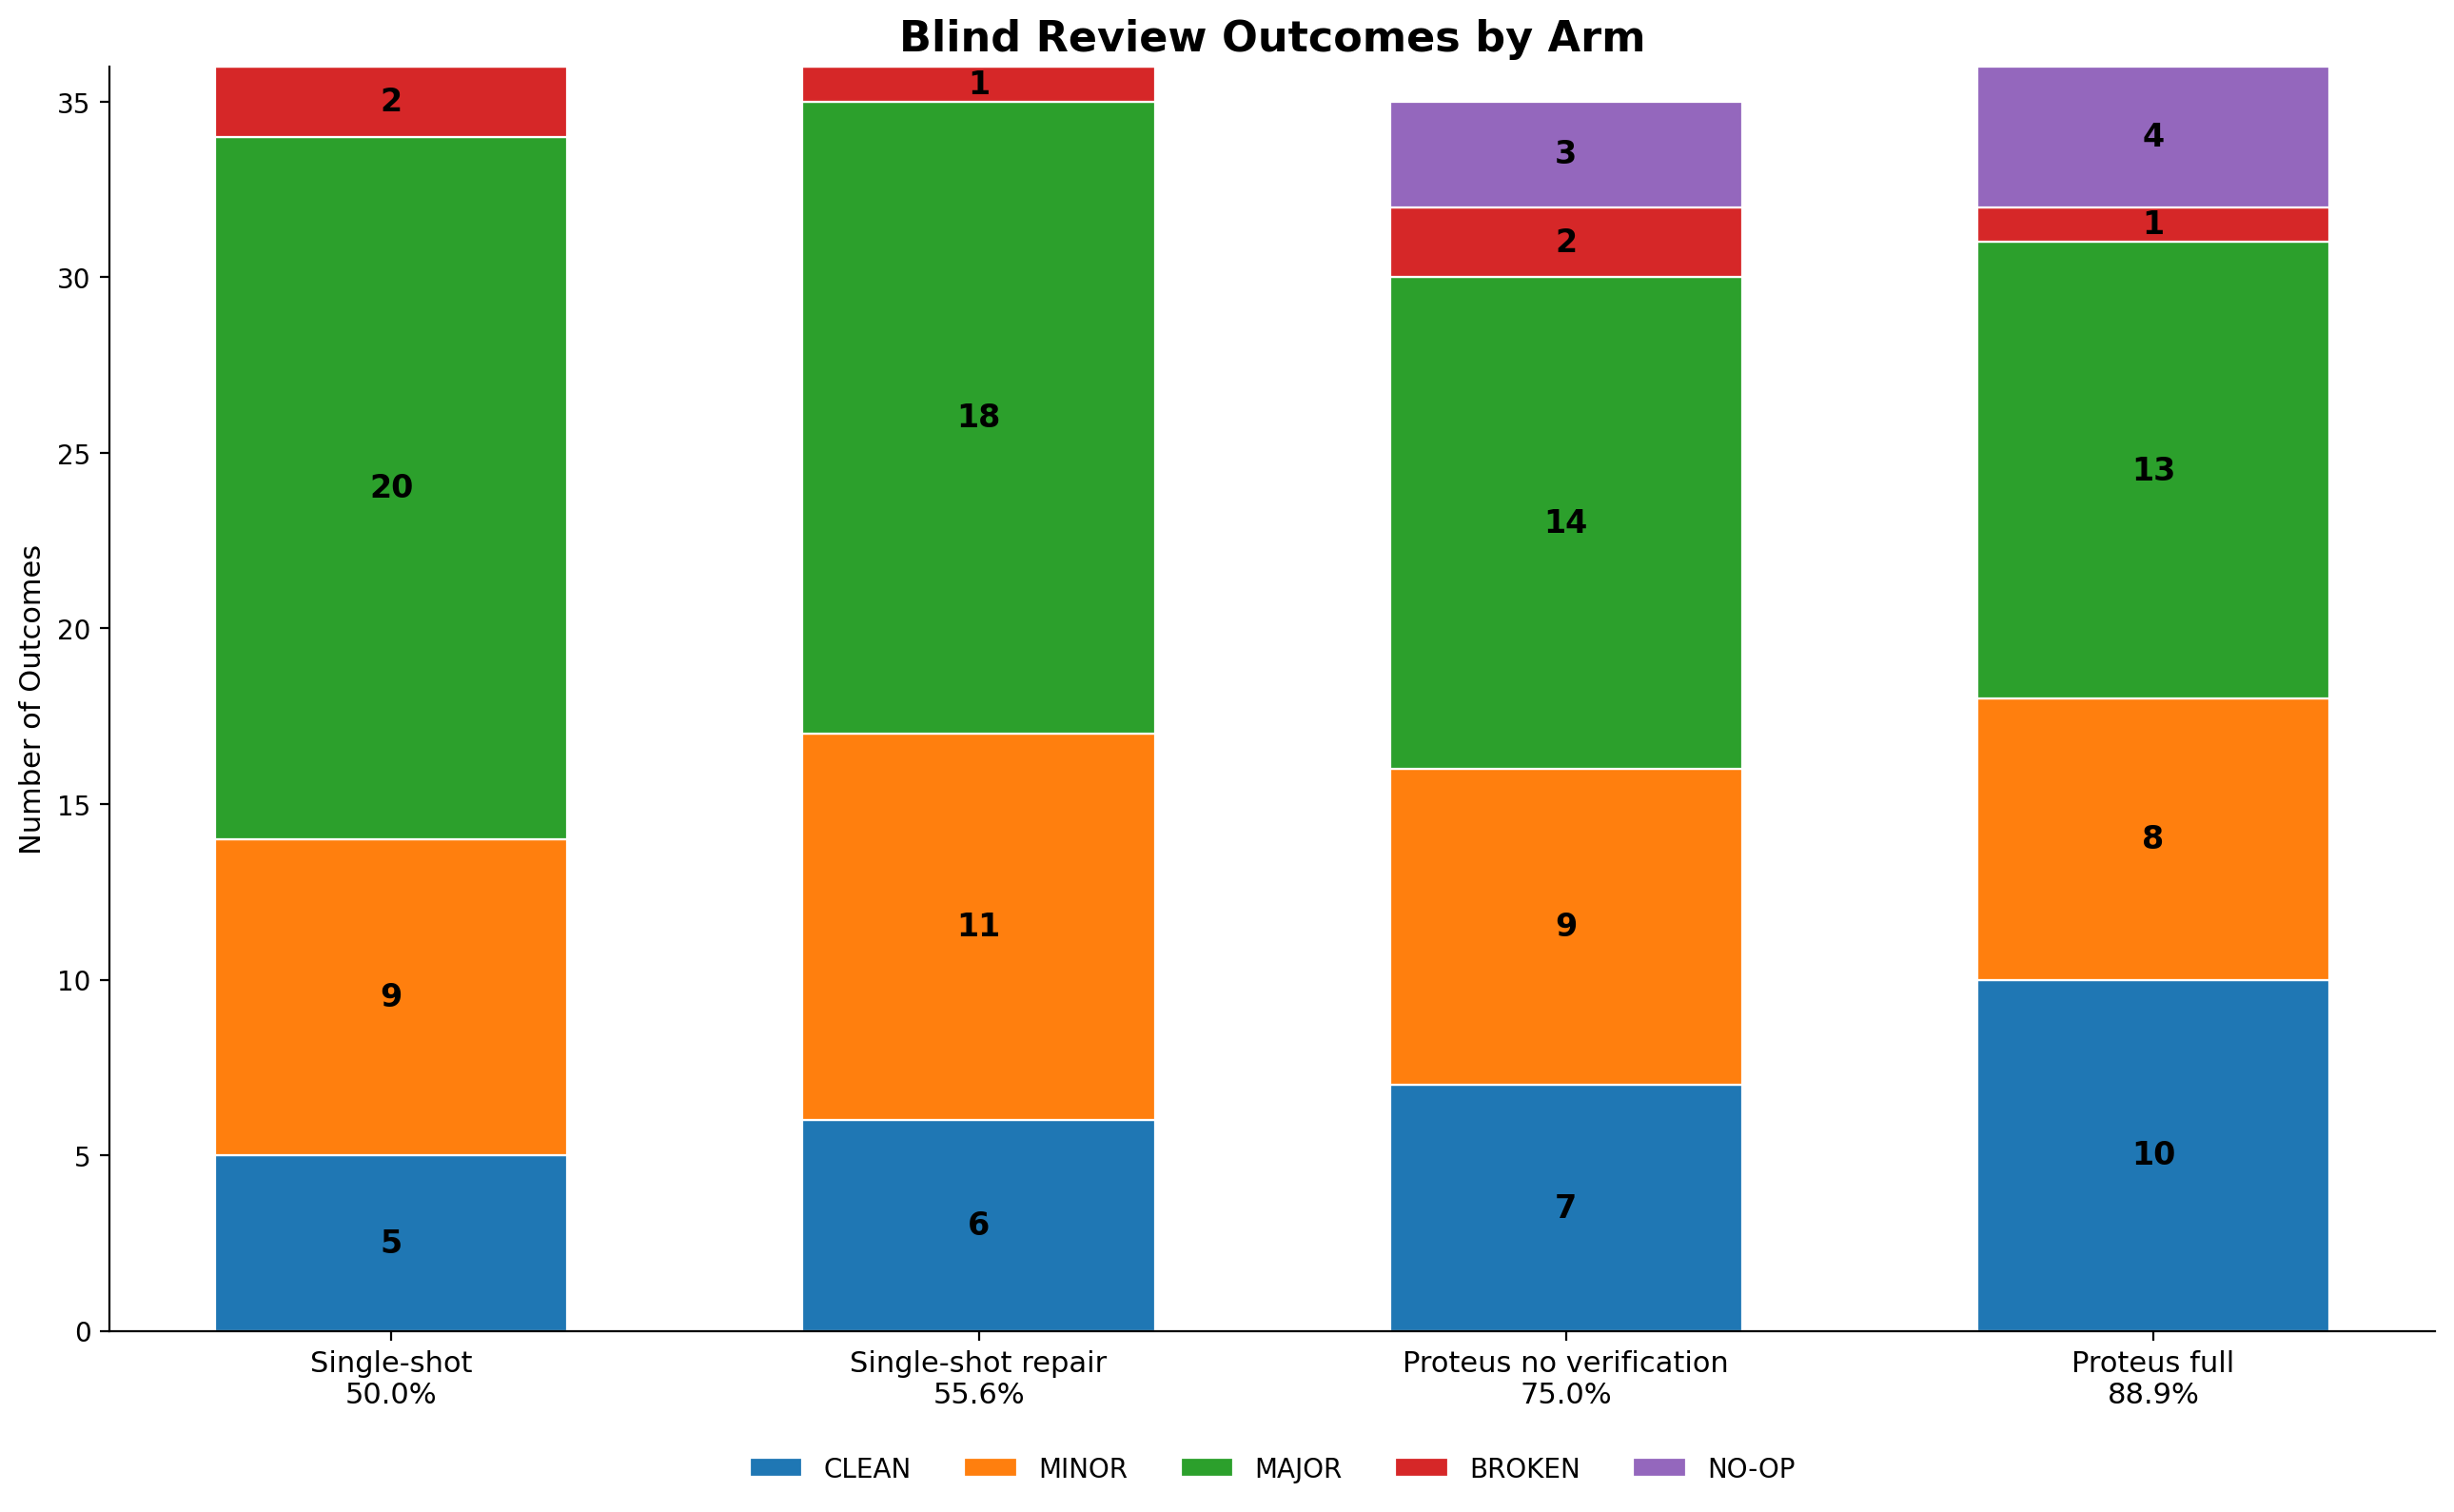
\includegraphics[width=\linewidth]{figs/blind_review_by_arm.png}
\caption{Every one of the 144 generated clones classified by the blind reviewer, stacked by configuration, with each configuration's migration success rate given below its bar. A \textsc{no-op} is counted as such whatever verdict it received: a clone that never migrated is trivially faithful to the original, so its \textsc{clean} carries no information. \emph{Takeaway:} migration success rises monotonically from single-shot (50.0\%) through single-shot-with-repair (55.6\%) and the no-verification ablation (75.0\%) to full \sys (88.9\%), and the \textsc{clean} share (blue) grows alongside it rather than being traded away for volume.}
\label{fig:results}
\end{figure}

Three observations follow.

First, \textbf{full \sys migrates far more often than every other configuration}. It succeeds on 32 of 36 runs, against 18 for the plain single-shot baseline and 20 for single-shot-with-repair — substantially ahead of both, and among the widest gaps of any comparison in this study.

Second, \textbf{full \sys leads on both ends of the blind reviewer's verdict distribution, in absolute terms}: it has both the most \textsc{clean} clones of any configuration (10, against 5 for the plain single-shot baseline) and the fewest \textsc{major}-or-\textsc{broken} clones of any configuration (14, against 22 for single-shot, 19 for single-shot-with-repair, and 16 for the ablation), despite attempting far more migrations than any of them. This holds even though full \sys's accepted pool is the largest of the four, which is the harder direction for a low absolute defect count to hold. We note this as a direction rather than an established effect: these \textsc{major}-or-\textsc{broken} counts are close enough across configurations (14, 16, 19, 22) that a different corpus could plausibly reorder them.

Third, \textbf{cost scales with recall}. Full \sys consumes roughly thirty-three times the tokens of the plain baseline (3.48M vs.\ 106K), at seventeen times its dollar cost (\$15.65 vs.\ \$0.92), and more than twice the ablation's tokens (3.48M vs.\ 1.43M) to convert that budget into 32/36 migrations against 27/36 and 18/36. The marginal spend over the ablation buys five additional migrations and a wider verification net (30 \emph{VCA}-triggered stage re-entries across the corpus, against none by construction for the ablation).

\textbf{A caution on small numbers.} With twelve subjects, most comparisons in this study beyond migration success itself are close enough that a different corpus could plausibly reorder them. Migration success is the one measure where the gap is wide enough to trust on its own, and only in the direction of full \sys over both single-shot baselines. We report the ablation comparison and the \textsc{clean}/\textsc{major}-\textsc{broken} counts above as directions worth noting, not established effects.

\subsection{Analysis}

\textbf{Which stage dominates repair cost.} Full \sys triggered 30 \emph{VCA} stage re-entries across 36 runs. The \emph{VCA} has two re-entry targets by construction: the \emph{Connector} when an adapter is wrong, and the \emph{LSA} when the selected library itself cannot satisfy the interface. The \emph{LMA} is not a repair target: its output is gated by the equivalence oracle before the \emph{VCA} observes it, so a rejected mutation is discarded rather than repaired. Repair iterations are capped at five per run; no run in this corpus exhausted that budget.

\textbf{Which requirement classes are hardest.} The two families of system fail differently in kind. The single-shot configurations drift semantically: a changed exception type or message, a client or connection never closed, a timeout or retry silently dropped, or a numeric-formatting edge case in the target library that the original never exhibited. Their wiring is usually correct where they attempt a change at all, but they attempt fewer changes and stop earlier. Full \sys fails at integration instead: an argument accepted by a generated adapter and then never used at the call site, a symbol imported from a plausible-but-wrong module path inside the new library, or a broad exception clause that catches a genuine defect alongside the failures it is meant to translate. Its adapters are structurally sound (generating a wrapper naturally preserves lifecycle and error translation), and the residual defects sit precisely at the seam between a correctly-designed adapter and the concrete surface of the real library.

\textbf{Characteristic failure modes, by verdict.} We illustrate the three non-trivial verdicts with one representative clone each, drawn directly from full \sys's output on this corpus (Section~\ref{sec:qualitative}). The \textsc{clean} case (\texttt{crc\_telemetry}, A1) shows a faithful drop-in replacement where the agent additionally normalizes an implementation-specific quirk the requirement did not ask about. The \textsc{minor} case (\texttt{iso\_ts\_parser}, A3) shows behavior that is correct on every input the test suite exercises but diverges in the exact wording of an error path on malformed input. The \textsc{major} case (\texttt{modbus\_meter\_reader}, B2) shows a clone that eagerly surfaces a connection failure the original silently deferred, a behavioral divergence visible only by comparing the two versions' own control flow, since the subject's own test suite injects a client whose connection always succeeds.

\textbf{What the global oracle catches.} Clones that import the migrated-to library while still calling the migrated-from one (a guaranteed \texttt{NameError} on the factory path) are rejected by the pipeline, at the \emph{LMA} or the \emph{VCA} depending on which agent introduced the reference, before ever reaching the blind reviewer. This is precisely the defect class the fifth oracle layer (factory execution against the real library) was added to catch: the first four layers never execute this path because every subject's own tests inject a fake client.

\subsubsection{Qualitative Examples}
\label{sec:qualitative}

To make the verdicts in Table~\ref{tab:judge} concrete, we reproduce full \sys clones drawn from the actual runs scored there, one for each of \textsc{clean}, \textsc{minor} and \textsc{major}, plus a second \textsc{clean} example chosen for high structural divergence. Each listing shows the essential diff against the pristine original; identifiers, structure and docstrings are exactly as \sys emitted them. Every claim quoted from the blind reviewer below was independently re-checked by us against the actually-installed target library or by direct execution, not taken on the reviewer's word alone; where a reviewer claim could \emph{not} be reproduced this way, we discarded that example rather than include it (see the note at the end of this subsection).

\paragraph{\textsc{Clean}: \texttt{crc\_telemetry} (A1, \texttt{zlib.crc32} $\rightarrow$ \texttt{fastcrc})}
The requirement is a bit-identical drop-in swap. \sys introduces a one-line wrapper that documents \emph{why} the mask is still applied even though the replacement already returns an unsigned value, rather than simply substituting the call:

\begin{lstlisting}[language=Python, basicstyle=\ttfamily\scriptsize, breaklines=true, frame=single]
-import zlib
+import fastcrc

+def _axiom_crc32_wrapper(payload: bytes) -> int:
+    """Compute a CRC-32 checksum of *payload*, matching zlib.crc32's
+    behavior. fastcrc.crc32.iso_hdlc implements the same CRC-32
+    algorithm (IEEE 802.3 / ISO-HDLC), and already returns an
+    unsigned integer, but we still apply the 0xFFFFFFFF mask here
+    to guarantee identical unsigned 32-bit normalization regardless
+    of any implementation-specific quirks.
+    """
+    return fastcrc.crc32.iso_hdlc(payload) & 0xFFFFFFFF

 def crc32(payload: bytes) -> int:
     """CRC-32 of *payload* as an unsigned 32-bit integer."""
-    return zlib.crc32(payload) & 0xFFFFFFFF
+    return _axiom_crc32_wrapper(payload)
\end{lstlisting}
The blind reviewer's verdict: \emph{``\texttt{fastcrc.crc32.iso\_hdlc} is the same CRC-32 (IEEE/ISO-HDLC) as \texttt{zlib.crc32}, the masking and all framing/verification logic including the \texttt{len<CRC\_LEN} boundary and validation error paths are unchanged.''} We independently confirmed this: \texttt{fastcrc.crc32.iso\_hdlc(p)} and \texttt{zlib.crc32(p)} return the identical integer for every payload we tried.

\paragraph{\textsc{Clean}, highly divergent: \texttt{telemetry\_gateway} (D3, \texttt{paho-mqtt} $\rightarrow$ \texttt{amqtt}, combined with first-party logic mutation)}
Category~D exercises all three transformation agents together, and this clone has the highest structural-divergence score of any \textsc{clean}-verdict clone in the corpus (composite divergence 0.536, against 0.026 for the drop-in \texttt{crc\_telemetry} example above). Rather than editing the smoothing logic in place, the \emph{LMA} extracts it into a new class in a new file, and re-exposes the original attributes as properties so every existing call site keeps working unchanged:

\begin{lstlisting}[language=Python, basicstyle=\ttfamily\scriptsize, breaklines=true, frame=single]
 # estimator.py
+from smoothing import MovingWindow

 class Estimator:
     def __init__(self, scale=0.1, window=5, roc_limit=5.0):
         self.scale = scale
-        self.window = window
         self.roc_limit = roc_limit
-        self.buffer = []
+        self._window_state = MovingWindow(window)
         self.last = None

+    @property
+    def buffer(self) -> list:
+        return self._window_state.values

     def update(self, raw_counts: float) -> dict:
         value = raw_counts * self.scale
-        self.buffer.append(value)
-        if len(self.buffer) > self.window:
-            self.buffer.pop(0)
-        smoothed = sum(self.buffer) / len(self.buffer)
+        smoothed = self._window_state.push(value)
         roc = 0.0 if self.last is None else abs(value - self.last)
         self.last = value
         return {"value": value, "smoothed": smoothed, "anomaly": roc > self.roc_limit}

+# smoothing.py -- new file
+class MovingWindow:
+    def __init__(self, size):
+        self.size = size
+        self.values = []
+    def push(self, value):
+        self.values.append(value)
+        if len(self.values) > self.size:
+            self.values.pop(0)
+        return sum(self.values) / len(self.values)
\end{lstlisting}
We did not rely on the reviewer's judgment alone for this one either: we extracted both the original list-based logic and the new \texttt{MovingWindow}-based logic and ran 5,000 random inputs through each side by side. Every output matched exactly.

The \texttt{estimator.py}/\texttt{smoothing.py} split shown above is only part of this clone's restructuring, not all of it. The same run adds two further new files on top of the three-file original: \texttt{estimator\_config.py}, a small \texttt{dataclass} bundling the estimator's construction parameters behind a \texttt{build\_estimator()} factory method, and \texttt{mqtt\_bridge.py}, a synchronous facade over \texttt{amqtt}'s async client, factored out of \texttt{sink.py} specifically so, in the clone's own docstring, ``the sync/async bridging plumbing can be reused or substituted independently of the sink's publishing logic.'' Three new files extracted from a three-file original is the largest structural reorganization any \textsc{clean}-verdict clone in this corpus makes, and it is exactly this kind of re-decomposition, not merely renaming, that the composite divergence score above is measuring.

\paragraph{\textsc{Minor}: \texttt{iso\_ts\_parser} (A3, \texttt{datetime.fromisoformat} $\rightarrow$ \texttt{ciso8601})}
Parsing itself is equivalent on every timestamp the test suite and the oracle exercise. The divergence is confined to the error path on malformed input:

\begin{lstlisting}[language=Python, basicstyle=\ttfamily\scriptsize, breaklines=true, frame=single]
-def parse(ts: str) -> datetime:
-    """Parse an ISO-8601 timestamp into a tz-aware datetime (UTC if naive)."""
-    dt = datetime.fromisoformat(_normalize(ts))
+def parse_datetime_utc_normalized(ts: str) -> datetime:
+    """ciso8601.parse_datetime accepts the trailing 'Z' zulu suffix
+    natively (no _normalize workaround needed) but likewise returns
+    a naive datetime when the input carries no UTC offset; attach
+    timezone.utc in that case to preserve this module's convention.
+    """
+    import ciso8601
+    dt = ciso8601.parse_datetime(ts)
     if dt.tzinfo is None:
         dt = dt.replace(tzinfo=timezone.utc)
     return dt

+def parse(ts: str) -> datetime:
+    """Parse an ISO-8601 timestamp into a tz-aware datetime (UTC if naive)."""
+    return parse_datetime_utc_normalized(ts)
\end{lstlisting}
The blind reviewer's verdict: \emph{``On malformed input the original raised \texttt{ValueError} from \texttt{datetime.fromisoformat} with a message like `Invalid isoformat string: ...'; \texttt{ciso8601.parse\_datetime} raises its own \texttt{ValueError} with a different message (and a \texttt{TypeError} rather than a \texttt{ValueError} for non-\texttt{str} input), so callers matching on message text would observe a difference confined to the malformed-input edge case.''} We independently confirmed this: both raise \texttt{ValueError} on the same malformed input, with different message text, exactly as described.

\paragraph{\textsc{Major}, migration success $=$ true, judge $\neq$ \textsc{clean}: \texttt{modbus\_meter\_reader} (B2, \texttt{pymodbus} $\rightarrow$ \texttt{pyModbusTCP})}
This clone received \texttt{migration\_success=true}: it compiled, its full suite passed, the oracle was satisfied, and the migration was genuine, yet the blind reviewer found a genuine behavioral change, and unlike the case below, this one does not depend on trusting any claim about a third-party library's undocumented internals; it is visible by reading the two versions of the program's own code side by side.

\begin{lstlisting}[language=Python, basicstyle=\ttfamily\scriptsize, breaklines=true, frame=single]
 def _default_client(host: str, port: int = 502):
-    from pymodbus.client import ModbusTcpClient  # lazy import
-    client = ModbusTcpClient(host, port=port)
-    client.connect()
+    client = _axiom_modbus_client_factory(host, port=port)
+    _axiom_modbus_connect_wrapper(client)
     return client

+def _axiom_modbus_connect_wrapper(client):
+    client.open()
+    if not client.is_open:
+        raise ConnectionError("Unable to connect to Modbus host")
+    return True
\end{lstlisting}
The original called \texttt{client.connect()} and discarded its boolean return value, so a construction-time connection failure was silent: the caller received a live-looking but disconnected client object, and the failure surfaced later, indirectly, wherever the first read happened to occur. The rewrite checks \texttt{client.is\_open} and raises \texttt{ConnectionError} immediately. This is not a defect in the sense of ``wrong'' (eagerly surfacing a connection failure is arguably better practice), but it is a genuine behavioral divergence the requirement did not ask for: any caller that relied on the original's silent-failure-then-later-IOError sequence (for example, code that retries transparently around \texttt{ModbusIO} construction) now sees a different exception, at a different point in the control flow, than the original ever raised. The subject's own tests inject a fake client whose \texttt{connect} always succeeds, so neither the pipeline's own verifier nor its test suite has any path that exercises the connection-failure branch on either side, which is exactly why an independent behavioral reviewer is needed to catch it.

\paragraph{A discarded example, and why}
An earlier draft of this subsection used a different Category~B clone (\texttt{mqtt\_telemetry\_bridge}, B3, \texttt{paho-mqtt}$\to$\texttt{amqtt}) whose reviewer finding turned on a specific claim about the installed \texttt{amqtt} library: that \texttt{ProtocolHandlerError} is not exported from \texttt{amqtt.client}. Checking this against the actually-installed \texttt{amqtt} 0.12.0 package, we found the claim false: \texttt{ProtocolHandlerError} \emph{is} defined directly in \texttt{amqtt.client}. Two further \textsc{major} findings on a different subject (\texttt{sensor\_json\_logger}, A2, concerning \texttt{ujson}'s default whitespace and non-ASCII handling) likewise did not reproduce against the installed \texttt{ujson} 5.12.1. We cannot tell, from the evidence available to us, whether these three findings are library-version drift between the original evaluation run and the machine we checked on, or reviewer error; either is possible, and we did not have a recorded pin of the exact library versions in place at evaluation time. Rather than present a reviewer claim we could not ourselves verify, we withdrew all three and report this instead: \emph{blind-review findings that turn on a specific claim about third-party library internals should be treated as provisional until independently checked against the exact library version in use, and we recommend any future use of this methodology pin and record that version at evaluation time.} The \texttt{modbus\_meter\_reader} example above was chosen deliberately to avoid this failure mode, because its defect is confined to code \sys itself wrote and needs no claim about \texttt{pyModbusTCP}'s internals to establish.

These clones illustrate a broader pattern: full \sys's adapters are consistently well-reasoned about \emph{intent} (why a mask is retained, why a naive datetime needs a timezone attached, why a moving-window class is reusable on its own), and the residual defects we could independently confirm are concentrated in the glue code's own control flow rather than in the first-party logic the \emph{LMA} rewrites.

\paragraph{\textsc{Lessons Learned}}
Three findings we did not anticipate.

\emph{Test suites are the wrong instrument for this task.} Dependency injection is good practice, and it makes the migrated code path untestable by the very suite that certifies it. Any future benchmark of clone generation needs an oracle that executes the substituted path directly, which is why we added factory execution as a fifth oracle layer mid-study, and why the \texttt{modbus\_meter\_reader} connection-handling defect above surfaces only under blind review.

\emph{Separating substitution from mutation keeps repairs local, but the seam leaks.} The \emph{LSA}/\emph{GSA} split behaves as intended (repairs stay within one agent, and no run in this corpus exhausted its repair budget), yet the residual failure mode lives precisely at the boundary, where an adapter is generated correctly and then relies on an assumption about the target library's surface that a static API-grounding check can catch but a purely execution-driven repair loop may not, if the failing line is never executed by available tests.

\emph{Verification changes how much is accepted, and how much of that is clean.} Disabling the \emph{VCA} changes both which clones clear acceptance at all (27/36 against 32/36) and, among those, how many the blind reviewer independently confirms as clean (7 against 10) or rates \textsc{major}-or-\textsc{broken} (16 against 14) in absolute terms, though at this corpus size neither gap is wide enough to trust as more than a direction. Recall is where the verification tier's contribution is best established in this evaluation.

\section{Discussion and Limitations}
\label{sec:limitations}

We frame \sys's limitations precisely and bound their scope.

\textbf{Un-evidenced repair on the reimplement-mode path.}
The First-Party Agent's own internal loop (Section~\ref{sec:looping}) is the only one of the four agents' local loops that includes a genuine behavioral check against golden vectors, not merely a static or syntactic one, and it is externally retried by the VCA exactly as the LSA and GSA are. Where it falls short of them is evidence: a wrapper-fixable or decision-level verdict against the LSA or GSA carries the concrete failure or an exclusion list into the next attempt, while the graph-level remapping that routes both verdicts to the First-Party Agent on this path carries nothing: the agent restarts its own five-attempt loop from the pristine source with no record of what the VCA rejected. On the two subjects in our corpus that exercise this path, all six runs across both configurations still reached an accepted migration (Table~\ref{tab:migration}), so the gap did not cost us a result here, but it is a real asymmetry in the implementation rather than a considered design choice, and closing it, threading the VCA's finding into the First-Party Agent's retry the way \texttt{\_last\_connector\_error} already does for the GSA, is a direct, low-risk next step.

\textbf{Oracle-bounded correctness.}
\sys certifies equivalence only up to the strength of its verification evidence. Behavioral equivalence is established over the available test corpus and the oracle's recorded vectors and invariants; it is not a formal proof. Consequently, an equivalence-confirmed clone is guaranteed equivalent \emph{on the exercised behaviors}, and residual divergence can persist on inputs neither the tests nor the oracle probes reach. This bound is well-understood and directly tied to test coverage: richer suites and traces tighten it, and the certification-heavy domains we target tend to supply exactly such assets. The blind review reported above is our attempt to probe outside that bound. It found \textsc{major} or \textsc{broken} defects among full \sys's accepted clones, and among every other configuration's, which is the sharpest available statement of how far the automated evidence falls short of the property it is taken to certify, even for the configuration with the highest recall.

The corpus's one \textsc{broken}-verdict full-\sys clone (\texttt{boiler\_control\_loop}, D1, \texttt{pymodbus}$\to$\texttt{pyModbusTCP}) illustrates exactly how the bound is exceeded. The migrated code calls \texttt{self.client.write\_register(address, counts, self.unit)}; \texttt{pyModbusTCP}'s real \texttt{ModbusClient} has no method named \texttt{write\_register} at all (we confirmed this directly by introspecting the installed package, which exposes \texttt{write\_single\_register} instead), so this call raises \texttt{AttributeError} on every real invocation. A second, independent defect in the same clone passes the Modbus unit id positionally into the position \texttt{read\_holding\_registers} uses for register \emph{count} (we confirmed the real signature is \texttt{read\_holding\_registers(reg\_addr, reg\_nb=1)}), silently corrupting a read whenever the unit id is not coincidentally equal to the intended register count of 1; on this corpus's own default configuration (\texttt{unit=1}) the two integers happen to coincide, so the defect is present but dormant. Neither defect is caught anywhere in the pipeline: the subject's own tests inject a fake client that defines \texttt{write\_register} under its old name and defaults its \texttt{unit} keyword to 1, so both bugs are invisible to the test suite by construction; and the fifth oracle layer, which calls the real factory against the reserved dead address \texttt{192.0.2.1} specifically to catch this class of defect, never reaches either bug either, because the connection attempt itself fails first and is correctly classified as \textsc{baseline} (inconclusive, both sides fail) rather than as a fault: the dead-address probe cannot distinguish ``failed because unreachable'' from ``would also have failed for a different reason further down the call path.'' This clone still received \texttt{migration\_success=true}: it compiled, its full suite passed, and the source-level oracle was satisfied. Only the blind review, which reads the migrated source rather than executing it against a live network, surfaced the defect at all. This is the concrete case for why we treat the automated acceptance signal as necessary but not sufficient, and why a production deployment of this methodology would need either a mocked-but-\emph{faithful} test double (one that raises on a call the real library does not support, rather than accepting it) or a fully live integration test, neither of which this corpus's dependency-injected design provides.

The same program, without the verification tier, fails differently rather than more safely. The no-verification ablation's own \texttt{boiler\_control\_loop} clone (D1, \texttt{pymodbus}$\to$\texttt{modbus\_tk}) extracts the Modbus glue into a separate \texttt{\_modbustk\_adapter.py}, whose \texttt{read\_holding\_registers} method correctly imports \texttt{socket}, \texttt{modbus\_tk.defines as cst}, and \texttt{modbus\_tk.modbus as modbus\_tk\_modbus} inside itself, but whose neighboring \texttt{write\_register} method references all three of those names with no import statement anywhere in its own scope, a plain \texttt{NameError} on the very first real write. \texttt{write\_valve()} calls this method directly on every actuation, so the bug sits on the hot path, not in a corner case. It is invisible for exactly the same structural reason as the full-\sys defect above: the subject's own tests inject a fake client and never reach \texttt{\_modbustk\_adapter.py} at all, and the fifth oracle layer's connection attempt to the reserved dead address fails before it ever reaches a write. This clone, too, received \texttt{migration\_success=true}. The two defects are not the same kind of mistake: one is a wrong method name inherited from a misremembered library surface, the other is a copy-paste omission between two sibling methods in code \sys wrote start to finish, with no third-party surface to misremember at all. That the verification tier's absence does not concentrate failure into one recognizable pattern, but instead lets whatever an agent happens to get wrong ship unchecked, is itself informative about what the tier is for.

\textbf{Scope of mutation.}
By construction the \emph{LMA} mutates only first-party logic, so the divergence \sys achieves is bounded by the ratio of first-party to third-party code in a subject program; dependency-dominated programs diversify primarily through substitution. The \emph{LSA} itself only selects \emph{among} existing libraries and cannot synthesize a first-party replacement; the two Category~C subjects whose requirement is precisely a substitution-to-first-party rewrite (\texttt{pid\_pump\_controller}, C1, and \texttt{tank\_level\_fsm}, C2) are instead routed to a separate First-Party Agent (Section~\ref{sec:fra}) that writes the removed dependency's behavior directly, and this evaluation's migration success on those two subjects (6/6 accepted across both, Table~\ref{tab:migration}) is that agent's, not the LSA's.

\textbf{Corpus scale and provenance.}
The twelve subjects are our own, authored for this study rather than harvested from public repositories. That costs external validity, and it is why the comparisons in Section~\ref{sec:results} that are not wide enough to stand on their own are reported as directions rather than established effects. It is also what makes per-program golden vectors and invariants available at all; without those the equivalence question cannot be posed at the granularity this study requires.

\textbf{Dual use.}
The ability to generate equivalent-but-divergent code is defensively valuable for diversification, but the same capability could aid evasion of similarity-based detection. We discuss this tension and the role of provenance reporting in Section~\ref{sec:conclusions}.
